% 短样张：展示 D 题最终工程的版式元素，文字仅保留结构所需的短段落。
% 公式、图表的具体写法见下文源码；正式论文请从 main.tex 开始。
\documentclass[withoutpreface]{gmcmthesis}
% 以 draft/D题/main.tex 为准；这里只抽出与论文内容无关的导言设置。
% 从 draft/D题 提取的统一表格样式；供所有三线表复用。
\newcolumntype{Y}[1]{>{\centering\arraybackslash}m{#1}}
\newcommand{\papertablestyle}{%
  \normalfont\songti\zihao{-4}%
  \linespread{1.15}\selectfont%
  \renewcommand{\arraystretch}{1}%
  \setlength{\tabcolsep}{5pt}%
  \setlength{\heavyrulewidth}{1pt}%
  \setlength{\lightrulewidth}{0.5pt}%
  \setlength{\aboverulesep}{3pt}%
  \setlength{\belowrulesep}{3pt}%
  \captionsetup{font={normalfont,song,minusfour},position=top,skip=4pt}%
}

\usepackage{fvextra,tcolorbox,pdfpages,eso-pic}
\tcbuselibrary{breakable}
\clubpenalty=10000
\widowpenalty=10000
\displaywidowpenalty=10000
\setCJKfamilyfont{abstractlisu}[Path=fonts/]{LiSu.ttf}
\geometry{footskip=13.82777pt}
\setcounter{tocdepth}{3}

\makeatletter
\def\@oddfoot{\hfill{\normalfont\fontsize{9bp}{11bp}\selectfont\thepage}\hfill}
\let\@evenfoot\@oddfoot
\newcommand\papertocline[4]{%
  \par\begingroup\normalfont\songti\fontsize{12bp}{18.6bp}\selectfont
  \leftskip=#1\relax\rightskip=12bp\parfillskip=-\rightskip
  \parindent=0pt\interlinepenalty=10000
  \@tempdima=#2\relax\advance\leftskip\@tempdima
  \leavevmode\hskip-\@tempdima{#3}\nobreak\hskip3bp
  \leaders\hbox to3bp{\hss.\hss}\hfill\nobreak
  \hb@xt@12bp{\hfil\normalfont\fontsize{12bp}{18.6bp}\selectfont#4}\par
  \endgroup}
\renewcommand\l@section[2]{\papertocline{0bp}{30bp}{#1}{#2}}
\renewcommand\l@subsection[2]{\papertocline{12bp}{21bp}{#1}{#2}}
\renewcommand\l@subsubsection[2]{\papertocline{24bp}{30bp}{#1}{#2}}
\renewcommand\tableofcontents{%
  \begingroup\normalfont\songti\fontsize{12bp}{18.6bp}\selectfont
  \setlength{\parskip}{0pt}\setlength{\parindent}{0pt}
  \vspace*{0bp}
  {\centering\fontsize{16.2bp}{20bp}\selectfont 目录\par}
  \vspace{2bp}\@starttoc{toc}\endgroup}
\makeatother

% 摘要页沿用 draft/D题 的矢量页眉，已从原页眉移除具体论文题目。
% 题目在原位置使用同一工程的宋体字号叠加；正文参数来自原 sections/abstract.tex。
\newenvironment{paperabstractpage}[1]{%
  \clearpage
  \newgeometry{left=70.8bp,right=69.676bp,top=70.8bp,bottom=91.29bp,footskip=34.2bp}%
  \begingroup\normalfont\songti\fontsize{12bp}{20.28bp}\selectfont
  \setlength{\parindent}{24bp}\setlength{\parskip}{0pt}\setlength{\topskip}{12bp}%
  \AddToShipoutPictureBG{\AtPageLowerLeft{
\includegraphics[width=\paperwidth,height=\paperheight]{assets/abstract-continuation.pdf}}}%
  \AddToShipoutPictureBG*{%
    \AtPageLowerLeft{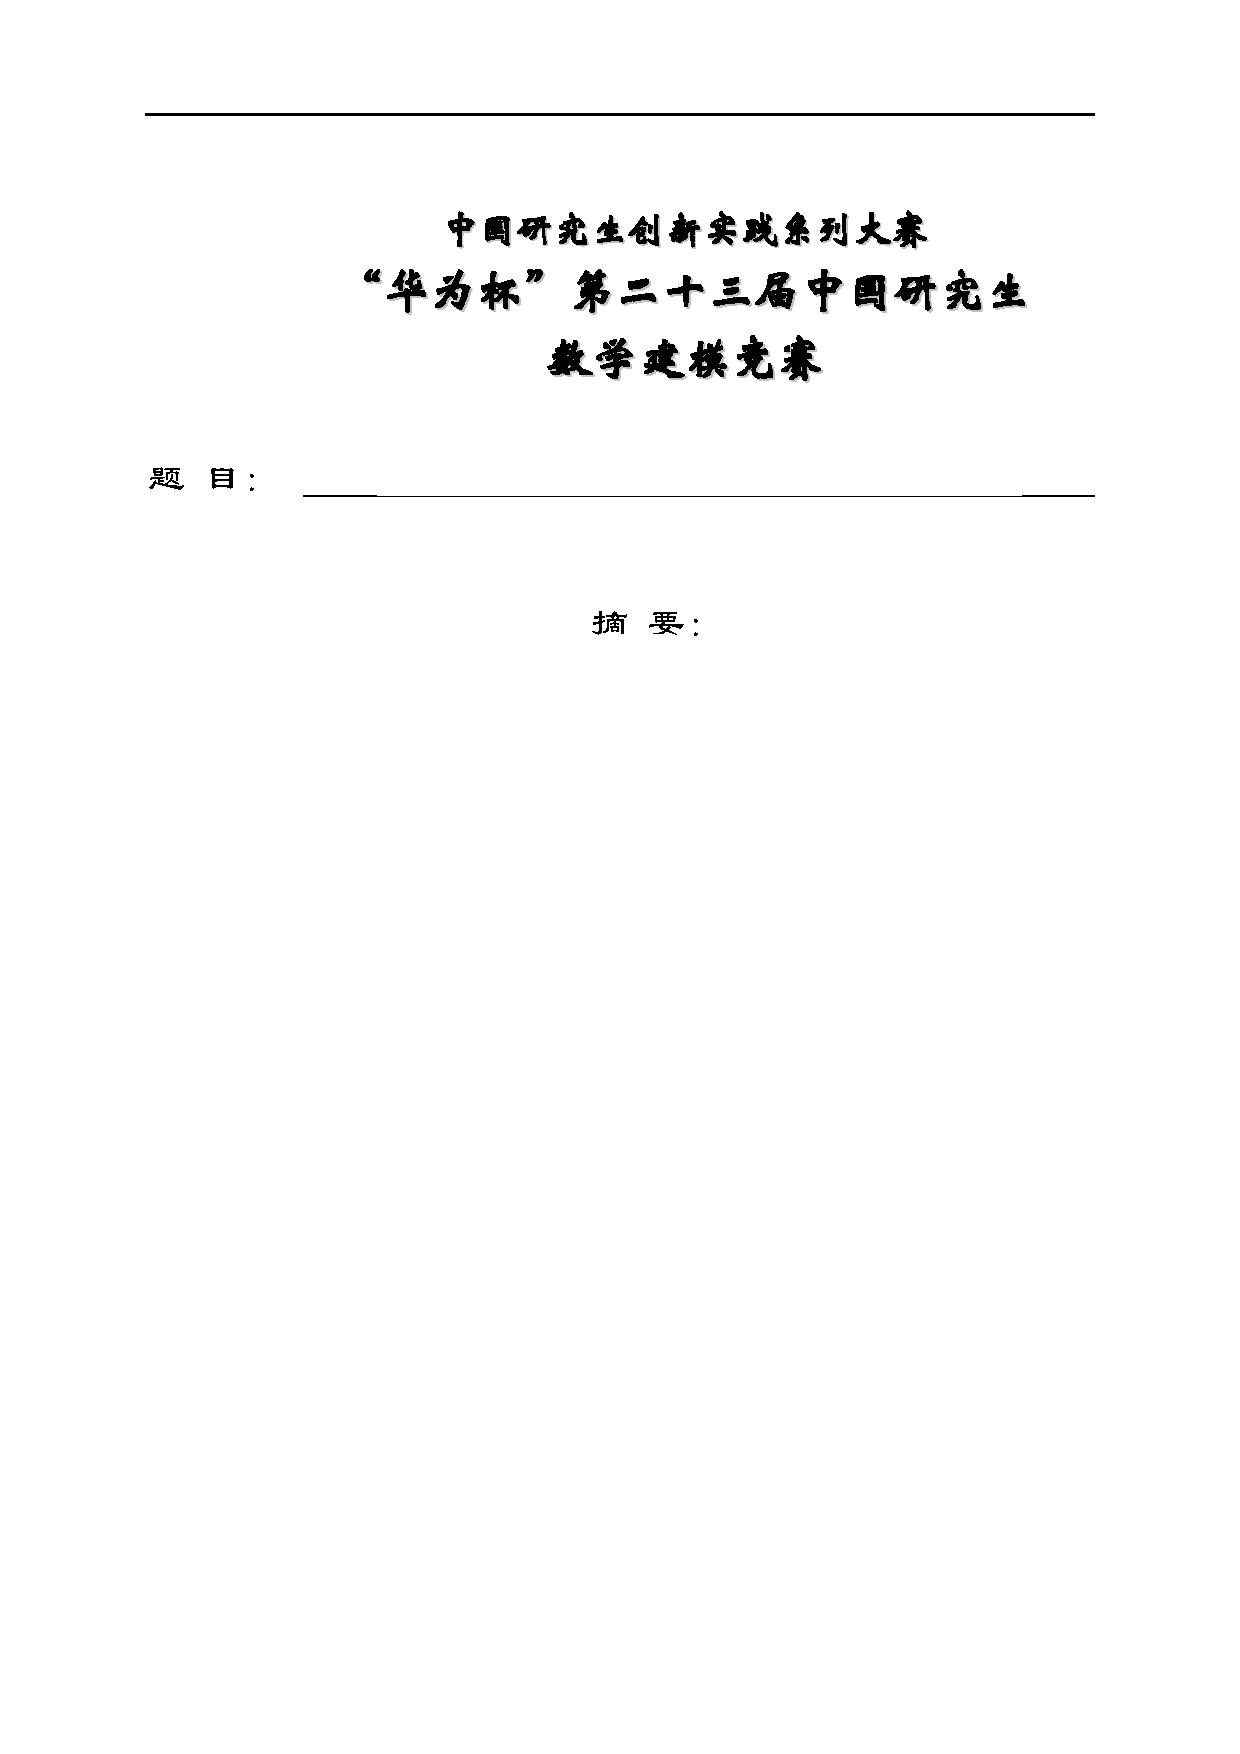
\includegraphics[width=\paperwidth,height=\paperheight]{assets/abstract-header.pdf}}%
    \AtPageUpperLeft{\put(181.8bp,-235.185bp){\heiti\fontsize{16.2bp}{18bp}\selectfont #1}}%
  }%
  \vspace*{231.12bp}%
}{%
  \par\clearpage\ClearShipoutPictureBG\endgroup\restoregeometry
}
\newcommand{\paperabstractkeywords}[1]{%
  \par\vspace{20.28bp}\noindent
  {\CJKfamily{abstractlisu}\fontsize{18bp}{20.28bp}\selectfont 关键词：}#1\par}

\hypersetup{pdftitle={数学建模论文排版示例},pdfauthor={},bookmarksopen=true}

\begin{document}
\pagenumbering{gobble}
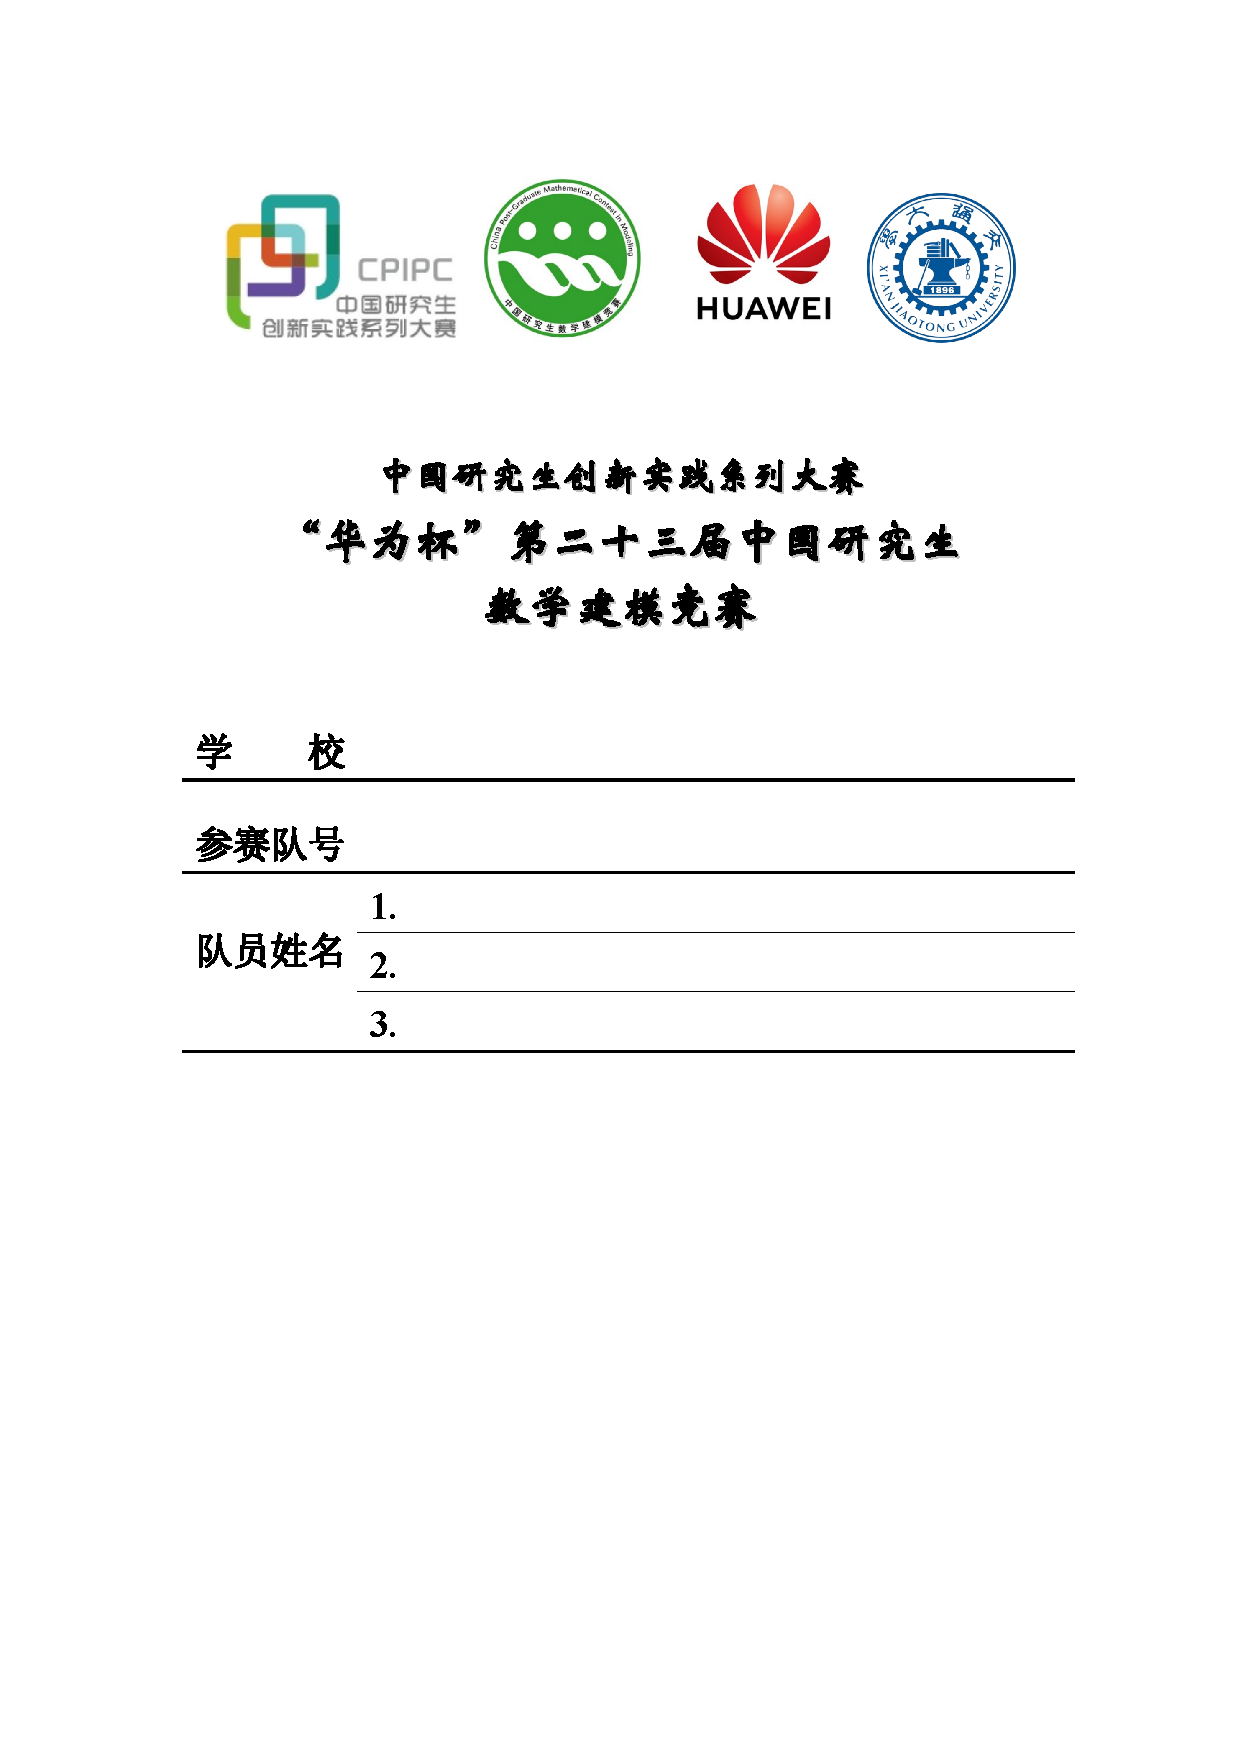
\includepdf[pages=1,pagecommand={\thispagestyle{empty}}]{assets/blank-cover.pdf}
\pagenumbering{arabic}

\begin{paperabstractpage}{山区洪涝灾害下无人机运输与通信协同优化}
山区洪涝灾害可能同时阻断道路与通信。为安排应急物资配送，需要综合考虑山区地形、无人机载荷、能源余量、货箱时限和连续通信保障。本文以单点往返、货箱组批、多点排程和中继协同为线索建立模型，并根据任务组独立执行的要求核算资源配置。

安全载荷由航线地形与返航电量共同限定；在此基础上筛选整箱装载模式，再按架次数、能耗和作业时间比较方案。多点运输与中继任务按设备和电池的占用时段协调安排。具体数值、求解过程与模型检验应在正式论文中完整报告。

\paperabstractkeywords{无人机运输；安全载荷；整箱组批；连续通信}
\end{paperabstractpage}

% 技术路线图在最终工程中位于摘要和目录之间，图号单列为“图1”。
% 此处只保留其位置；正式论文替换为研究过程生成的技术路线图。
\clearpage
\tableofcontents
\clearpage

\Needspace{94pt}
\section{问题重述}
\subsection{问题背景}
洪涝灾害造成道路受损后，分散居民点的补给任务需要无人机参与。运输能力同时受到地形净空、装载容量与能源储备的限制，通信受山体遮挡时还须安排中继保障。
\subsection{问题提出}
依次确定单点往返的安全载荷与整箱组批、多点多架次运输安排、连续通信条件下的中继调度，以及独立任务组的资源配置。

\Needspace{94pt}
\section{模型假设与符号说明}
\subsection{模型假设}
货箱完整交付，不拆分运输；单架次的载货质量和体积均不超过机型限制。运输机与电池分别记录可用时刻，返航后保留规定的安全余量。
\subsection{符号说明}
以 $g$ 表示运输机型，$q$ 表示所载货物质量。主要符号见表\ref{tab:symbols}；各问题专用变量在相应模型中定义。

\Needspace{130pt}
\begingroup
\papertablestyle
\setlength{\LTpre}{6pt}
\setlength{\LTpost}{6pt}
\begin{longtable}{@{}Y{36mm}Y{100mm}Y{15mm}@{}}
\caption{主要符号说明}\label{tab:symbols}\\
\toprule
符号 & 含义 & 单位 \\
\midrule
\endfirsthead
\caption[]{主要符号说明（续）}\\
\toprule
符号 & 含义 & 单位 \\
\midrule
\endhead
\bottomrule
\endfoot
$Q_g$ & 机型 $g$ 的最大载货质量 & kg \\
\addlinespace[5pt]
$L_g^0,L_g^F$ & 空载与满载标准航程 & km \\
\addlinespace[5pt]
$L_g(q)$ & 载荷 $q$ 下的等效航程 & km \\
\addlinespace[5pt]
$\rho_g$ & 返航安全余量比例 & — \\
\end{longtable}
\endgroup

\Needspace{94pt}
\section{数据预处理}
\subsection{输入与核对}
附件给出节点坐标、数字高程模型、逐箱需求、设备性能和通信参数。整理时保留原始编号与单位，检查箱号、服务区归属、质量、体积和时限字段。

\Needspace{94pt}
\section{问题一模型的建立与求解}
\subsection{问题分析}
先由往返航线的地形与能量预算确定各机型的安全载荷，再筛选满足质量、体积和返航约束的整箱装载模式。山区往返与组批的关系见图\ref{fig:route}。

\paperfigure[140mm]{examples/round-trip-and-batching.pdf}{山区单点往返与整箱组批示意}{fig:route}

图\ref{fig:route}中的载货去程与空载返程沿同一路径飞行；图示仅帮助说明运输过程，参数仍以赛题附件为准。

\subsection{单点往返运输模型的建立与求解}
\subsubsection{往返能耗模型}
按给定关系，机型 $g$ 在载荷 $q$ 下的等效航程计算公式如下：
\nopagebreak[4]
\begin{equation}\label{eq:range}
L_g(q)=L_g^0-(L_g^0-L_g^F)\left(\frac{q}{Q_g}\right)^{3/2}
\qquad 0\le q\le Q_g
\end{equation}
其中，$L_g^0$、$L_g^F$ 分别为空载和满载标准航程，$Q_g$ 为额定载货质量。根据式\eqref{eq:range}计算去程水平能耗时，需使用该架次的实际载荷。

\Needspace{200pt}
\subsection{货箱组批结果分析}
不同目标优先次序下的组批方案见表\ref{tab:batch}。架次数优先与能耗优先的方案构成两种权衡选择。
\begin{table}[H]
\centering
\papertablestyle
\caption{不同目标优先次序下的组批结果}\label{tab:batch}
\begin{tabular}{@{}Y{55mm}Y{20mm}Y{31mm}Y{43mm}@{}}
\toprule
优先次序 & 架次数 & 总能耗/kWh & 累计作业时间/min \\
\midrule
架次数、能耗、时间 & 18 & 59.131296 & 546.267 \\
\addlinespace[5pt]
能耗、架次数、时间 & 19 & 59.033942 & 574.000 \\
\bottomrule
\end{tabular}
\end{table}

能耗优先方案比架次数优先方案增加1架次，同时降低总能耗；选择时需结合运输时间与设备周转要求。

\section{参考文献}
\noindent [1] 依据实际阅读和引用的文献填写。\par
\appendix
\section{补充材料}
此处可列推导、代码清单或补充表格。
\end{document}
